\documentclass[dvipdfmx]{jsarticle}
\usepackage[dvipdfmx]{graphicx}
\usepackage{amsmath, amssymb}
\usepackage{mathtools}
\usepackage{here}
\begin{document}
\title{週間進捗報告}
\author{権藤陸}
\date{2022年5月20日}
\maketitle
\section{進捗}
いただいた論文を読み進めた.
\section{PPGセンサの原理 \cite{ppg}}
PPGセンサは.血液によって吸収・反射される赤外線の量を測定する.受光される光の波長は約940nmである.センサには透過型・反射型の2種類が存在する.透過型のPPGセンサでは,LEDの光は皮膚の色素や骨,動脈血や静脈血等の吸収性物質を透過し,フィルタやコンバータ通し,光検出器で光エネルギーを計測する.一方,反射型のセンサは,LED光を皮膚で反射させ,それを検出器で受光し,フィルタやコンバータで同様に定量化する.
よって,PPG波形は主に血液量の変化に起因し,光エネルギーの減衰変化を表す.
より具体的には,PPGは血液中のグルコースによって生じる光散乱の特性に基づいている.グルコースが増加すると,その存在によって屈折率が低下するため,組織を透過する光ビームの位置ずれが減少する.その結果,吸収される光量が少なくなり,組織を通過する光強度が大きくなる.PPG技術は、光強度が吸収性媒体中を進むと指数関数的に減少し,吸収は波長に依存することを示すBeer-Lambertの法則に基づいている.

PPG信号は直流と交流成分の2つの成分から形成される.直流成分は,組織を通過する光の一定の吸収を表すDCオフセット,交流成分は光が動脈を通過するときに血液量の変化によって生成される成分である.

% \begin{figure}[htbp]
% \begin{center}
% \includegraphics[width=\linewidth]{filePath}
% \end{center}
% \caption{title}
% \end{figure}

\section{関連研究}
\subsection{従来の機械学習によるBP予測}
\begin{itemize}
    \item PPG信号から特徴量を網羅的に抽出
    \item FFTに基づくPPG信号の振幅と位相情報から1朴ごとの血圧を予測
    \item 血液の密度や粘性率,心拍数や収縮期の血管径心拍数を用いた新たな特徴量Womersley numberを使用
    \item アルゴリズムとしては,MLP,SVM,ランダムフォレスト,決定木が用いられる
\end{itemize}
\subsection{深層学習によるBP予測}
\begin{itemize}
    \item 時間領域と周波数領域の入力に対し,完全畳込みネットワークを用いる手法
    \item 手作業で取得した特徴量を用い,LSTM層を複数重ねたDeepRNNモデルを用いる手法
    \item ドメイン敵対学習を導入した,LSTMベースのマルチタスク回帰ネットワークを用いる手法
\end{itemize}
\subsection{ABP波形予測}
\begin{itemize}
    \item BP波形を直接予測した研究はほとんどない.
    \item UNetをディープスーパービジョンの概念と組み合わせ,PPG信号からABP波形を生成
    \item LeNetとUNetをそれぞれABP波形予測モデル構築に適用
\end{itemize}
\section{RDAE(Regularized Deep AutoEncoder)}
本研究では,ディープオートエンコーダに,ドメイン敵対学習の考えを取り込んだRDAEを提案する.RDAEが最適化すべき損失関数は以下のような形で表される.
\begin{equation}
    l(\phi, \varphi, \pi) = \mathrm{E}_{(x, y) \sim P_{data}} L_r(D_{\varphi} (E_{\phi}(x)), y) - \lambda \cdot L_d (D_\pi (E_{\phi} (x)), d_x)
\end{equation}
第一項は信号変換損失を表し$L_r ()$はMAEである.第二項はドメイン分類樹に対する分類損失を表し,$L_d ()$はソフトマックスロスである.$\lambda $は2項の重みをトレードオフするハイパーパラメータである.エンコーダのパラメータ$\phi$は勾配降下法により,
\begin{equation}
    \phi \leftarrow \phi - \alpha \cdot \nabla_{\phi} (L_r - \lambda \cdot L_d)
\end{equation}
のように更新される.$L_r$は信号変換損失,$L_d$はドメイン分類器の損失のため,敵対的に学習される.

RDAEのネットワーク構成は,CNNベースでエンコーダ4層,デコーダ4層となっている.

\begin{figure}[htbp]
\begin{center}
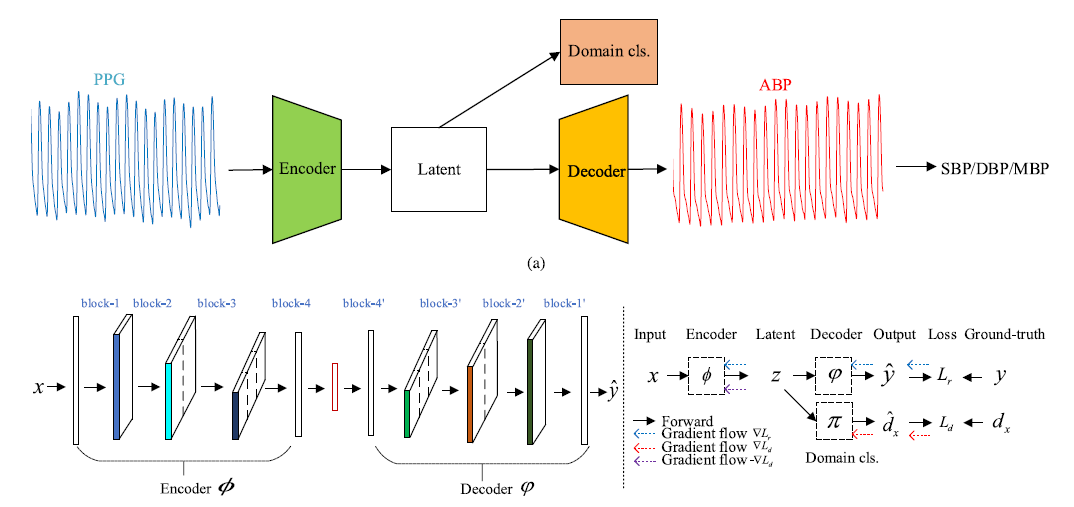
\includegraphics[width=\linewidth]{./rdae_model.png}
\end{center}
\caption{RDAEの構成とパラメータ}
\end{figure}
\section{結果}
収縮期血圧(SBP),拡張期血圧(DBP)平均血圧(MBP)予測において,キャリブレーションを行わない段階におけるRDAEのMAEはそれぞれ,7.945, 4.114, 3.834mmHgを達成した.
また,80秒のキャリブレーションを行った後のRDAEのMAEは5.424, 3.144, 2.885mmHgを達成した.
他の手法との比較の図は以下のようになった.
\begin{figure}[htbp]
\begin{center}
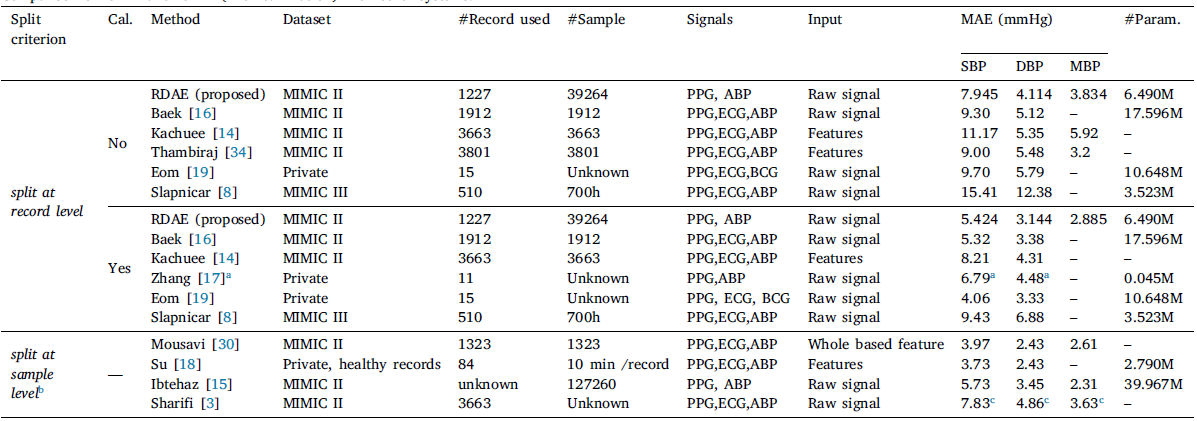
\includegraphics[width=\linewidth]{./result_comparison_with_other_system.png}
\end{center}
\caption{他の手法との結果の比較}
\end{figure}

キャリブレーションを行わない場合のSBPのMAE(表の1行目:RDAE(proposed))は7.945mmHgで他の手法よりも明らかに高い精度で予測できていることが分かる.
また,キャリブレーションを行った場合のSBPのMAE(表の7行目:RDAE(proposed))は,Baekらの手法に約1.4mmHgほど劣る値となっているが,Baekらは半分のテストサンプルを用いてキャリブレーションを行っているのに対し,提案手法では4分の1のテストサンプルしか用いていないためと考えられる.
また,BaekらやEomらの手法はMAEの値が提案手法に優っているが,パラメータのサイズは提案手法の方がずっと小さいものとなっている.
表の下4行の結果はデータをサンプルレベルで分割したアプローチであり,上12行の結果よりも良い結果が出ているが,これはデータリーケージの恐れがあるためと考えられる.

以上より,血圧予測精度とパラメータサイズにおいて,本手法は他の手法よりも優れたモデルであるといえる.

\section{計画}
発表の日程(または次のミーティング)までに,

発表スライドの作成,

本論文・関連研究のさらなる読み込みを行う.

\begin{thebibliography}{}
    \bibitem{ppg} Moraes, J. L., Rocha, M. X., Vasconcelos, G. G., Vasconcelos Filho, J. E., De Albuquerque, V. H. C., and Alexandria, A. R. (2018). Advances in photopletysmography signal analysis for biomedical applications. Sensors, 18(6), 1894.
\end{thebibliography}
% &を直接書くとエラーになるので注意
% \bibliographystyle{jplain} %参考文献出力スタイル
% \bibliography{week4} %hoge.bibから拡張子を外した名前
\end{document}